In this section, will be present
the case where the coronary 
artery has atherosclerosis and 
the drug-eluting stent is placed. 
It is modeled by 10 uniformly spaced 
semi-circles. 
The geometry used promotes a smooth reduction of the 
distance between the upper wall and symmetry axis of the channel. 
Due to atherosclerosis, 40\% channel obstruction was considered 
and the domain was discretized using 15875 nodes and 35408 
linear triangular elements. 

\par 
The \ref{velocity evolution curved stent} shows the unsteady velocity 
profile in the position where the horizontal velocity has maximum
non-dimensional value ($x=5.35R$). 
As we can see, the maximum non-dimensional value of the velocity field 
reaches $u=3.5$ when the stent is placed, that is, 
more than 3 times the blood velocity
in coronary artery.

\begin{figure}[H]
     \centering
     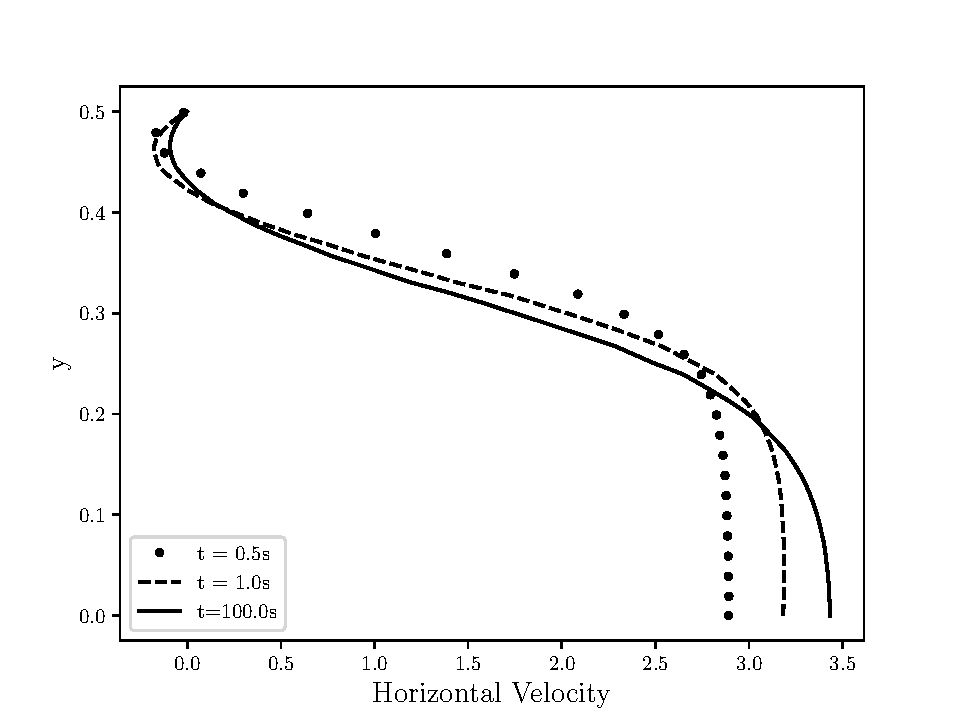
\includegraphics[scale=1]{./02_chaps/cap_solution/figure/vel_CurvedStrut_evol.pdf}\\
     \caption{
The unsteady velocity profile for curved channel with drug-eluting stent.}
     \label{velocity evolution curved stent}
\end{figure}

\newpage
The \ref{velocity field curved stent} presents the evolution in 
time and space of the velocity field for half of the domain. 
The velocity field is represented with non-dimensional values 
where the red color refers to the $u=3.5$ value and the blue color 
$u=0$ value. Conveting to dimensional values, 
we have $u=42cm/s$ and $u=0cm/s$ respectively.

\vspace{2cm} 
\begin{figure}[H]
     \begin{minipage}{.50\linewidth}
      \centering
      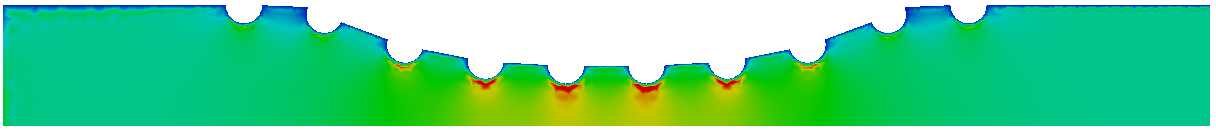
\includegraphics[scale=0.18]{./02_chaps/cap_solution/figure/vel_CurvedStrut1.png}\\
      t = 0.1
     \end{minipage}%
     \begin{minipage}{.50\linewidth}
      \centering
      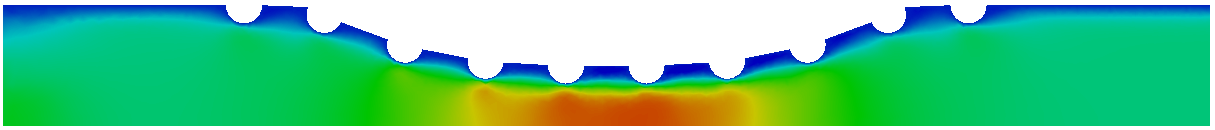
\includegraphics[scale=0.18]{./02_chaps/cap_solution/figure/vel_CurvedStrut2.png}\\
      t = 0.5
     \end{minipage}
     \begin{minipage}{.50\linewidth}
     \medskip
      \centering
      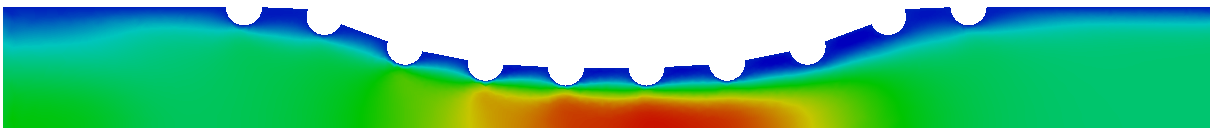
\includegraphics[scale=0.18]{./02_chaps/cap_solution/figure/vel_CurvedStrut3.png}\\
      t = 1.0
     \end{minipage}%
     \begin{minipage}{.50\linewidth}
     \medskip
      \centering
      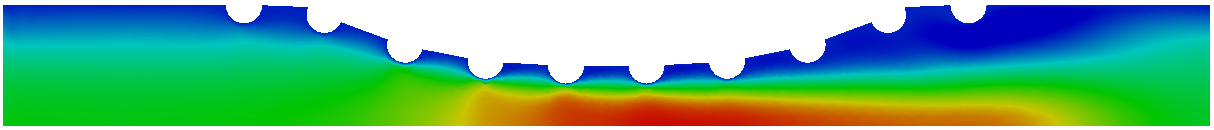
\includegraphics[scale=0.18]{./02_chaps/cap_solution/figure/vel_CurvedStrut4.png}\\
      t = 3.0
     \end{minipage}
     \begin{minipage}{.50\linewidth}
      \centering
      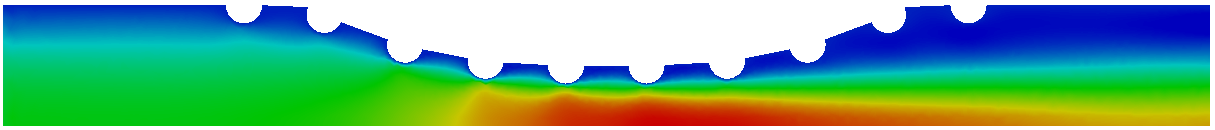
\includegraphics[scale=0.18]{./02_chaps/cap_solution/figure/vel_CurvedStrut5.png}\\
      t = 5.0
     \end{minipage}%
     \begin{minipage}{.50\linewidth}
      \centering
      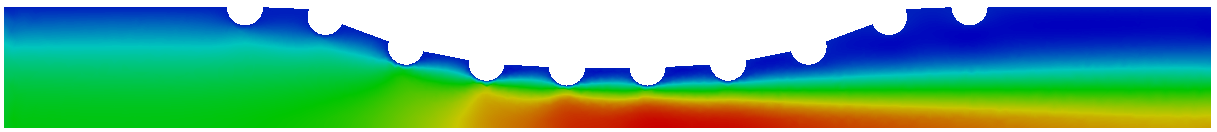
\includegraphics[scale=0.18]{./02_chaps/cap_solution/figure/vel_CurvedStrut6.png}\\
      t = 7.0
     \end{minipage}
     \begin{minipage}{.50\linewidth}
     \medskip
      \centering
      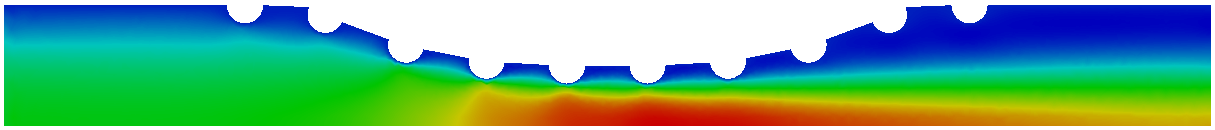
\includegraphics[scale=0.18]{./02_chaps/cap_solution/figure/vel_CurvedStrut7.png}\\
      t = 10.0
     \end{minipage}%
     \begin{minipage}{.50\linewidth}
     \medskip
      \centering
      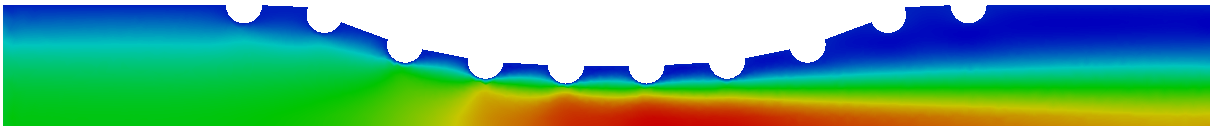
\includegraphics[scale=0.18]{./02_chaps/cap_solution/figure/vel_CurvedStrut8.png}\\
      steady state
     \end{minipage}\\[10pt]
      \centering
      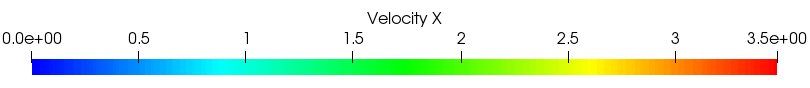
\includegraphics[scale=0.5]{./02_chaps/cap_solution/figure/vel_CurvedStrutScale.png}\\
     \medskip
     \caption{
Time and space evolution of the velocity field for curved channel with
drug-eluting stent.}
     \label{velocity field curved stent}
\end{figure}


\vspace{1cm}
As mentioned by Lucena et al. (2018) \cite{lucena2018}, 
it is estimated that 47\% of the drug is diffused to the 
lumem and it is lost to the bloodstream.
The \ref{conc field curved stent sc 1} and 
\ref{conc field curved stent sc 10} show the time and space evolution 
of the concentration field for several \textit{Schmidt} number, 
such as: $1$, $10$, $100$ and $1000$ respectively. The concentration field is 
represented with the non-dimensional values where the red color 
represents $100$\% and the blue color represents $0$\% 
of the diffused concentration in the bloodstream. 
It is possible to observe that the \textit{Schmidt} number directly 
influences the drug transport in the blood flow. 
For high values of the \textit{Schmidt} number, 
the transport of chemical species becomes purely convective.



\begin{figure}[H]
     \begin{minipage}{.50\linewidth}
      \centering
      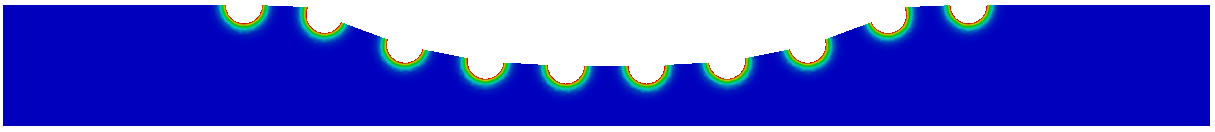
\includegraphics[scale=0.18]{./02_chaps/cap_solution/figure/conc1_CurvedStrut1.png}\\
      t = 0.1
     \end{minipage}%
     \begin{minipage}{.50\linewidth}
      \centering
      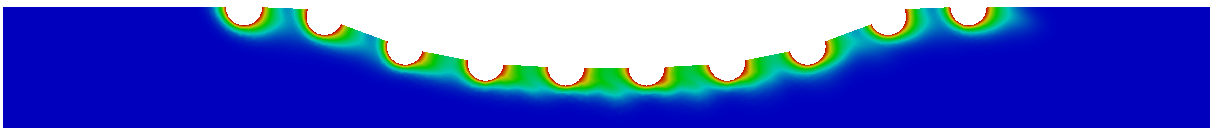
\includegraphics[scale=0.18]{./02_chaps/cap_solution/figure/conc1_CurvedStrut2.png}\\
      t = 0.5
     \end{minipage}
     \begin{minipage}{.50\linewidth}
     \medskip
      \centering
      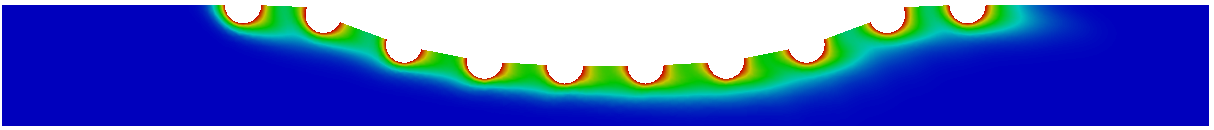
\includegraphics[scale=0.18]{./02_chaps/cap_solution/figure/conc1_CurvedStrut3.png}\\
      t = 1.0
     \end{minipage}%
     \begin{minipage}{.50\linewidth}
     \medskip
      \centering
      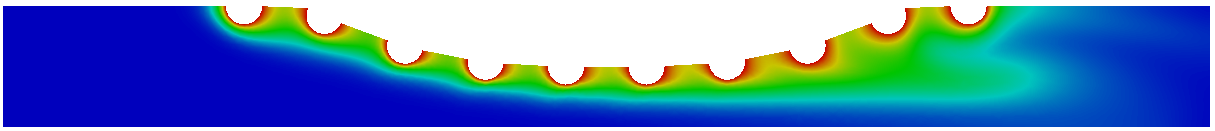
\includegraphics[scale=0.18]{./02_chaps/cap_solution/figure/conc1_CurvedStrut4.png}\\
      t = 3.0
     \end{minipage}
     \begin{minipage}{.50\linewidth}
      \centering
      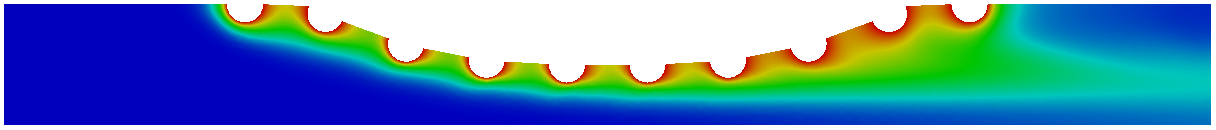
\includegraphics[scale=0.18]{./02_chaps/cap_solution/figure/conc1_CurvedStrut5.png}\\
      t = 5.0
     \end{minipage}%
     \begin{minipage}{.50\linewidth}
      \centering
      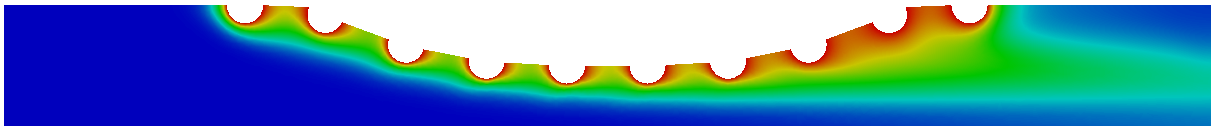
\includegraphics[scale=0.18]{./02_chaps/cap_solution/figure/conc1_CurvedStrut6.png}\\
      t = 7.0
     \end{minipage}
     \begin{minipage}{.50\linewidth}
     \medskip
      \centering
      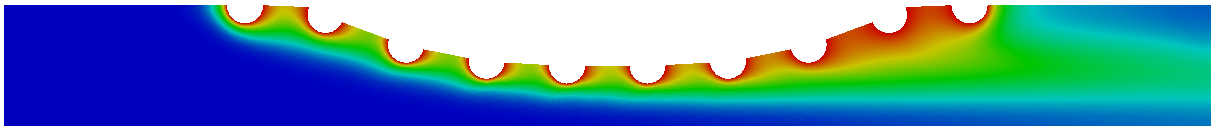
\includegraphics[scale=0.18]{./02_chaps/cap_solution/figure/conc1_CurvedStrut7.png}\\
      t = 10.0
     \end{minipage}%
     \begin{minipage}{.50\linewidth}
     \medskip
      \centering
      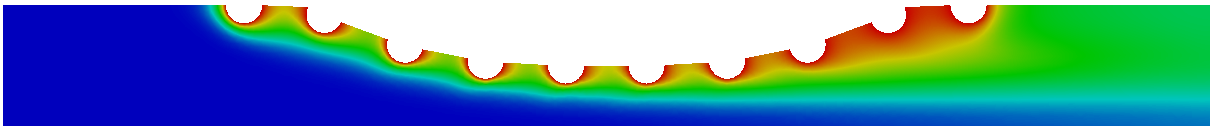
\includegraphics[scale=0.18]{./02_chaps/cap_solution/figure/conc1_CurvedStrut8.png}\\
      steady state
     \end{minipage}\\[10pt]
      \centering
      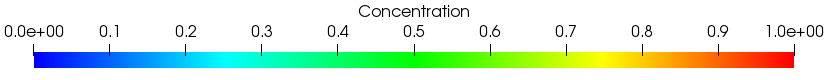
\includegraphics[scale=0.5]{./02_chaps/cap_solution/figure/conc1_CurvedStrutScale.png}\\
     \medskip
     \caption{
Time and space evolution of the concentration fiel for curved channel with drug-eluting stent with $Sc=1$.}
     \label{conc field curved stent sc 1}
\end{figure}



\begin{figure}[H]
     \begin{minipage}{.50\linewidth}
      \centering
      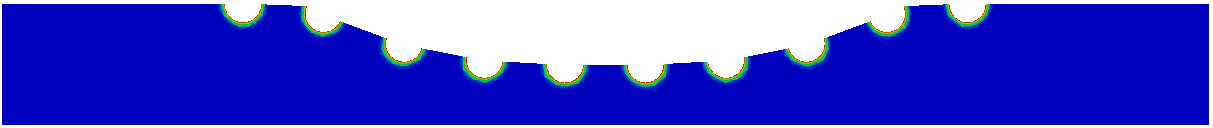
\includegraphics[scale=0.18]{./02_chaps/cap_solution/figure/conc10_CurvedStrut1.png}\\
      t = 0.1
     \end{minipage}%
     \begin{minipage}{.50\linewidth}
      \centering
      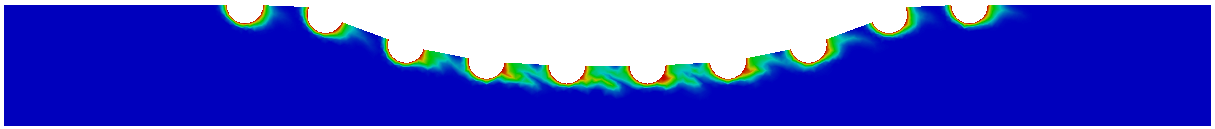
\includegraphics[scale=0.18]{./02_chaps/cap_solution/figure/conc10_CurvedStrut2.png}\\
      t = 0.5
     \end{minipage}
     \begin{minipage}{.50\linewidth}
     \medskip
      \centering
      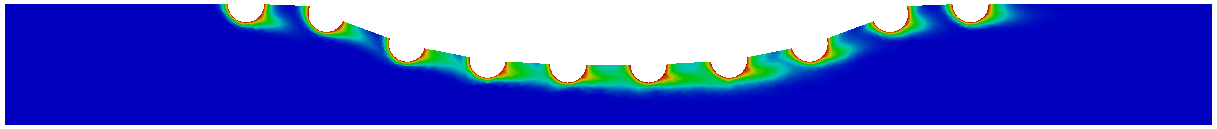
\includegraphics[scale=0.18]{./02_chaps/cap_solution/figure/conc10_CurvedStrut3.png}\\
      t = 1.0
     \end{minipage}%
     \begin{minipage}{.50\linewidth}
     \medskip
      \centering
      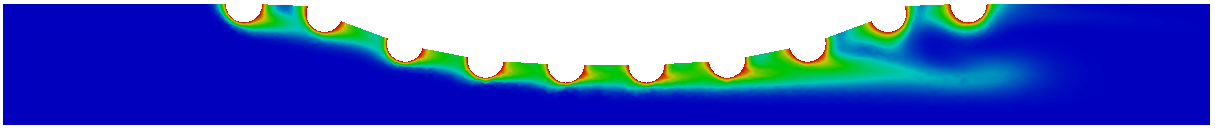
\includegraphics[scale=0.18]{./02_chaps/cap_solution/figure/conc10_CurvedStrut4.png}\\
      t = 3.0
     \end{minipage}
     \begin{minipage}{.50\linewidth}
      \centering
      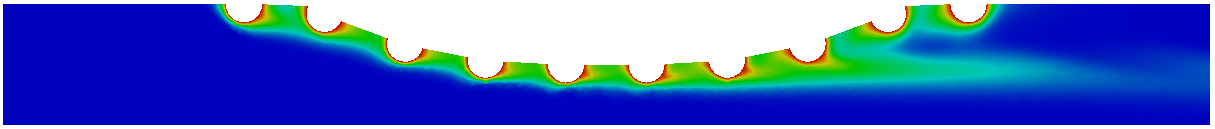
\includegraphics[scale=0.18]{./02_chaps/cap_solution/figure/conc10_CurvedStrut5.png}\\
      t = 5.0
     \end{minipage}%
     \begin{minipage}{.50\linewidth}
      \centering
      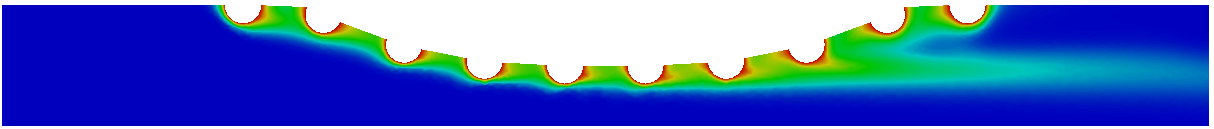
\includegraphics[scale=0.18]{./02_chaps/cap_solution/figure/conc10_CurvedStrut6.png}\\
      t = 7.0
     \end{minipage}
     \begin{minipage}{.50\linewidth}
     \medskip
      \centering
      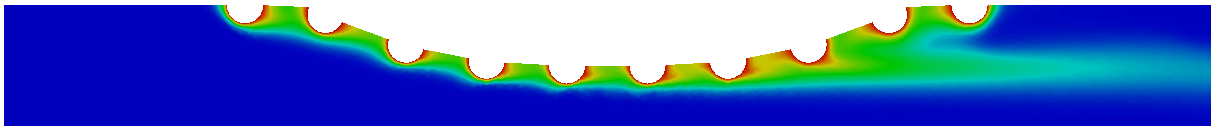
\includegraphics[scale=0.18]{./02_chaps/cap_solution/figure/conc10_CurvedStrut7.png}\\
      t = 10.0
     \end{minipage}%
     \begin{minipage}{.50\linewidth}
     \medskip
      \centering
      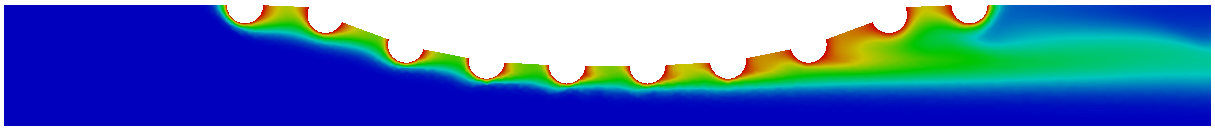
\includegraphics[scale=0.18]{./02_chaps/cap_solution/figure/conc10_CurvedStrut8.png}\\
      steady state
     \end{minipage}\\[10pt]
      \centering
      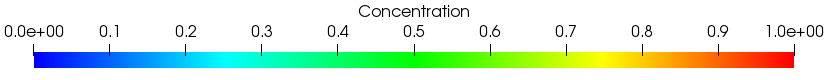
\includegraphics[scale=0.5]{./02_chaps/cap_solution/figure/conc1_CurvedStrutScale.png}\\
     \medskip
    \caption{
Time and space evolution of the concentration fiel for curved channel with drug-eluting stent with $Sc=10$.}
     \label{conc field curved stent sc 10}
\end{figure}



\begin{figure}[H]
     \begin{minipage}{.50\linewidth}
      \centering
      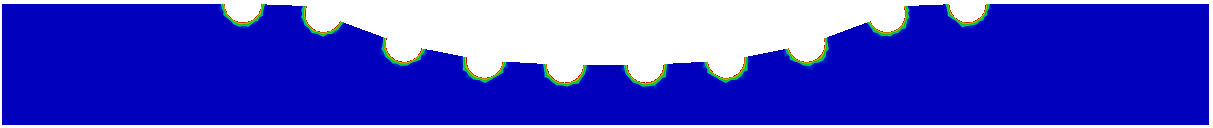
\includegraphics[scale=0.18]{./02_chaps/cap_solution/figure/conc100_CurvedStrut1.png}\\
      t = 0.1
     \end{minipage}%
     \begin{minipage}{.50\linewidth}
      \centering
      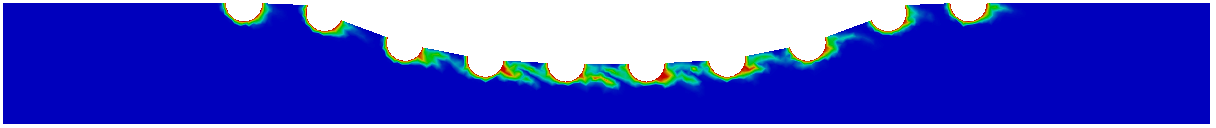
\includegraphics[scale=0.18]{./02_chaps/cap_solution/figure/conc100_CurvedStrut2.png}\\
      t = 0.5
     \end{minipage}
     \begin{minipage}{.50\linewidth}
     \medskip
      \centering
      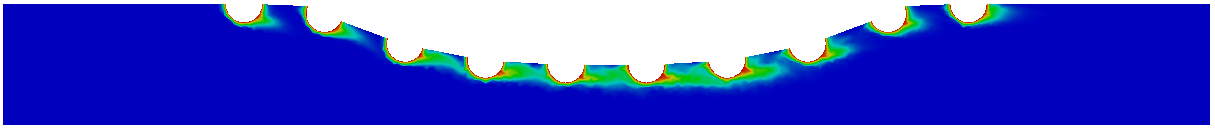
\includegraphics[scale=0.18]{./02_chaps/cap_solution/figure/conc100_CurvedStrut3.png}\\
      t = 1.0
     \end{minipage}%
     \begin{minipage}{.50\linewidth}
     \medskip
      \centering
      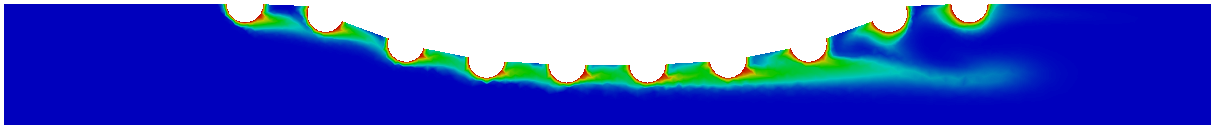
\includegraphics[scale=0.18]{./02_chaps/cap_solution/figure/conc100_CurvedStrut4.png}\\
      t = 3.0
     \end{minipage}
     \begin{minipage}{.50\linewidth}
      \centering
      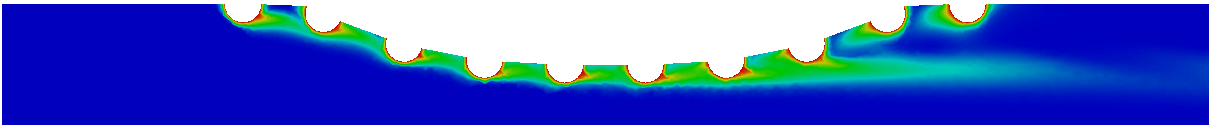
\includegraphics[scale=0.18]{./02_chaps/cap_solution/figure/conc100_CurvedStrut5.png}\\
      t = 5.0
     \end{minipage}%
     \begin{minipage}{.50\linewidth}
      \centering
      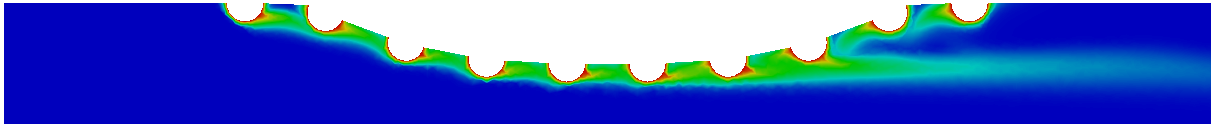
\includegraphics[scale=0.18]{./02_chaps/cap_solution/figure/conc100_CurvedStrut6.png}\\
      t = 7.0
     \end{minipage}
     \begin{minipage}{.50\linewidth}
     \medskip
      \centering
      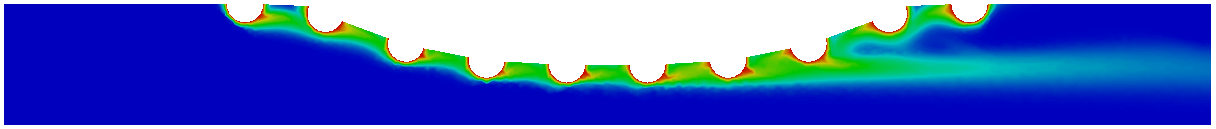
\includegraphics[scale=0.18]{./02_chaps/cap_solution/figure/conc100_CurvedStrut7.png}\\
      t = 10.0
     \end{minipage}%
     \begin{minipage}{.50\linewidth}
     \medskip
      \centering
      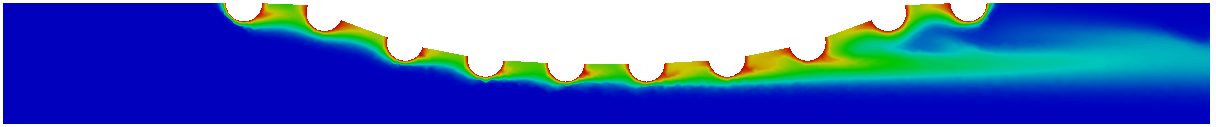
\includegraphics[scale=0.18]{./02_chaps/cap_solution/figure/conc100_CurvedStrut8.png}\\
      steady state
     \end{minipage}\\[10pt]
      \centering
      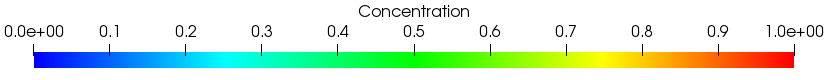
\includegraphics[scale=0.5]{./02_chaps/cap_solution/figure/conc1_CurvedStrutScale.png}\\
     \medskip
    \caption{
Time and space evolution of the concentration fiel for curved channel with drug-eluting stent with $Sc=100$.}
     \label{conc field curved stent sc 100}
\end{figure}

\begin{figure}[H]
     \begin{minipage}{.50\linewidth}
      \centering
      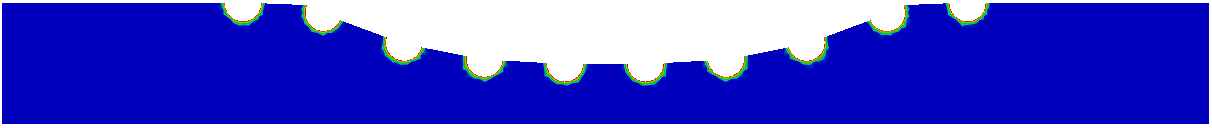
\includegraphics[scale=0.18]{./02_chaps/cap_solution/figure/conc1000_CurvedStrut1.png}\\
      t = 0.1
     \end{minipage}%
     \begin{minipage}{.50\linewidth}
      \centering
      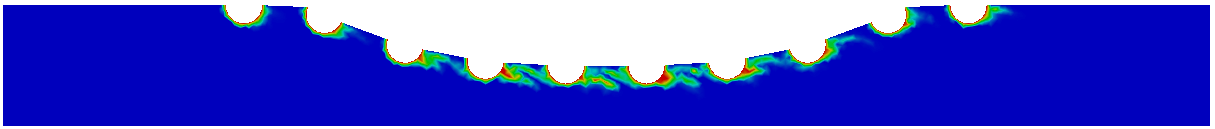
\includegraphics[scale=0.18]{./02_chaps/cap_solution/figure/conc1000_CurvedStrut2.png}\\
      t = 0.5
     \end{minipage}
     \begin{minipage}{.50\linewidth}
     \medskip
      \centering
      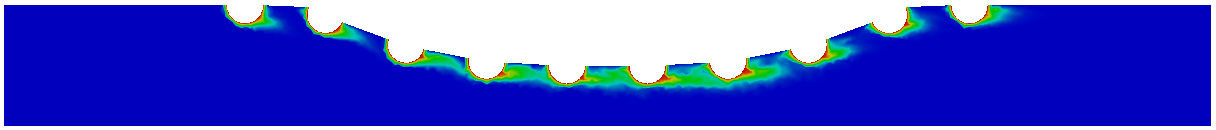
\includegraphics[scale=0.18]{./02_chaps/cap_solution/figure/conc1000_CurvedStrut3.png}\\
      t = 1.0
     \end{minipage}%
     \begin{minipage}{.50\linewidth}
     \medskip
      \centering
      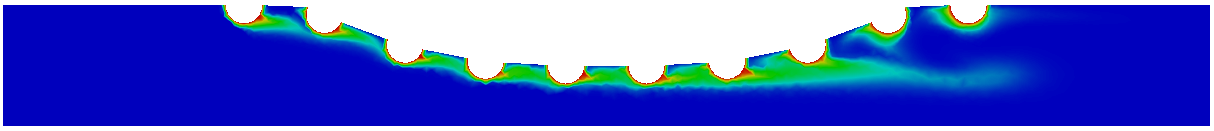
\includegraphics[scale=0.18]{./02_chaps/cap_solution/figure/conc1000_CurvedStrut4.png}\\
      t = 3.0
     \end{minipage}
     \begin{minipage}{.50\linewidth}
      \centering
      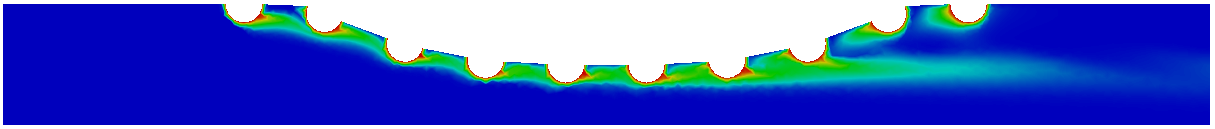
\includegraphics[scale=0.18]{./02_chaps/cap_solution/figure/conc1000_CurvedStrut5.png}\\
      t = 5.0
     \end{minipage}%
     \begin{minipage}{.50\linewidth}
      \centering
      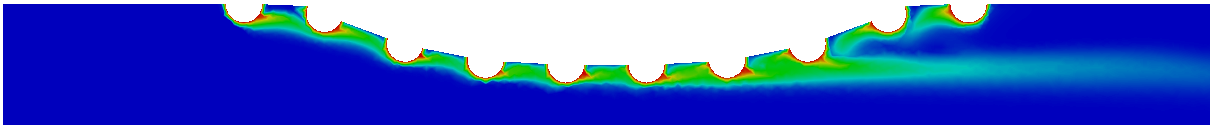
\includegraphics[scale=0.18]{./02_chaps/cap_solution/figure/conc1000_CurvedStrut6.png}\\
      t = 7.0
     \end{minipage}
     \begin{minipage}{.50\linewidth}
     \medskip
      \centering
      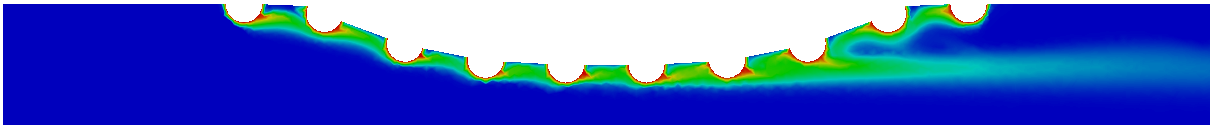
\includegraphics[scale=0.18]{./02_chaps/cap_solution/figure/conc1000_CurvedStrut7.png}\\
      t = 10.0
     \end{minipage}%
     \begin{minipage}{.50\linewidth}
     \medskip
      \centering
      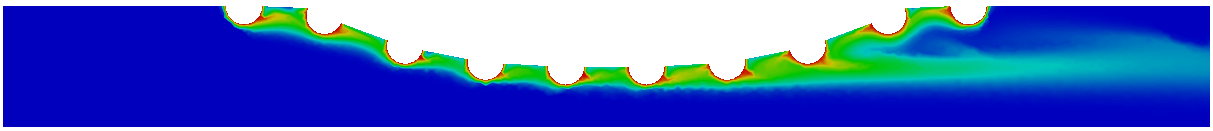
\includegraphics[scale=0.18]{./02_chaps/cap_solution/figure/conc1000_CurvedStrut8.png}\\
      steady state
     \end{minipage}\\[10pt]
      \centering
      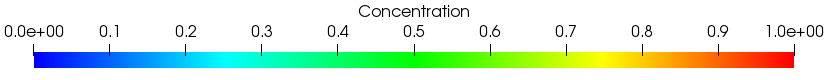
\includegraphics[scale=0.5]{./02_chaps/cap_solution/figure/conc1_CurvedStrutScale.png}\\
     \medskip
    \caption{
Time and space evolution of the concentration fiel for curved channel with drug-eluting stent with $Sc=1000$.}
     \label{conc field curved stent sc 1000}
\end{figure}


